\section{Bayesian Network}

Determining the correct action to trigger based on the contextual information is done using a Bayesian network. In this section, we will describe key aspects of a Bayesian network.

A Bayesian network is modelled as a graph which is composed of nodes and edges between the nodes. Each node in the network represents a variable and edges connect two nodes. If there is a causal relationship between two nodes, the edge is directed. If there is only some correlation between two nodes, the edge is undirected \cite{stephenson2000introduction}.

Two nodes, A and C are said to be conditionally independent if there is no edge between them. If we introduce a variable B and directed edges from B to A and B to C, both A and B are said to be dependent on B. B is totally independent because it does not depend on other nodes where as A and B are said to be conditionally independent given B \cite{stephenson2000introduction}. The network is illustrated in figure \cref{fig:analysis:bayesian-network:abc}.

\begin{figure}[h!]
\centering
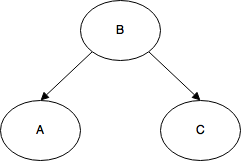
\includegraphics[width=0.3\textwidth]{images/a_b_c_bayesian_network}
\caption{Simple Bayesian network. The network consist of three nodes, i.e. three variables: A, B and C. A and C depends on B and B is totally independent \cite{stephenson2000introduction}.}
\label{fig:analysis:bayesian-network:abc}
\end{figure}

For each variable in the Bayesian network there is a probability distribution function which depends on the edges leading into the variable. Probability distribution functions can be illustrated using \emph{probability tables}. A probability table is said to be \emph{conditional}, i.e. it is a \emph{conditional probability table} if the variable to which the table belongs depends on one or more variables.

Probabilities are denoted $P(A|B)$, meaning the probability of A given B. An alternative notation is $P(A=a|B=b)$, meaning the probability of variable $A$ having value, also referred to as being \emph{in state}, $a$ when $B$ is in state $b$. $P(A|B,C) = P(A|B)$ when A and C are conditionally independent as is the case in \cref{fig:analysis:bayesian-network:abc}. The joint distribution of nodes, $X = X_1,\ldots,X_n$, in a network is 

\begin{equation}
\label{eq:analysis:bayesian-network:prod}
P(X) = \displaystyle \prod_{i=1}^{n} P(X_i|parents(X_i))
\end{equation}

In case of the network illustrated in \cref{fig:analysis:bayesian-network:abc}, the joint distribution of all variables is

\begin{equation}
P(A, B, C) = P(A|B) \cdot P(B) \cdot P(C|B)
\end{equation}

We also have that if the node $x_0$ does not depend on $x_n$, then we can remove $x_n$ when calculating the probability of $x_0$ as shown in \cref{eq:analysis:bayesian-network:not-child} \cite{stephenson2000introduction}.

\begin{equation}
\label{eq:analysis:bayesian-network:not-child}
P(x_0|x_1,\ldots,x_n,\ldots,x_k) = P(x_0|x_1,\ldots,x_{n-1},x_{n+1},\ldots,x_k)
\end{equation}

A graphical model of a Bayesian network consists of $K$, a set of nodes, $E$ a set of edges between the nodes and $P$, a set of probability distributions for each variable \cite{stephenson2000introduction}. In case of \cref{fig:analysis:bayesian-network:abc} $K = \{A, B, C\}$ and $E = \{\{B, A\}, \{B,C\}\}$. An example definition of $P$ can be the probability table and conditional probability tables shown in \cref{tbl:analysis:bayesian-network:abc-tables}. For example, the tables show that $P(B=Yes) = 0.3$ and $P(A=No|B=Yes) = 0.8$. This is the \emph{prior distribution}, i.e. our beliefs before any evidence is observed.

\begin{table}[h!]
\centering
\caption{Sample probability table and conditional probability tables for nodes A, B and C in the network illustrated in \cref{fig:analysis:bayesian-network:abc}.}
\label{tbl:analysis:bayesian-network:abc-tables}
\begin{tabular}{ccc}
\begin{tabular}{c}
\textbf{B}   \\
\begin{tabular}{cc}
Yes   & No \\ \hline
0.3 & 0.7
\end{tabular}
\end{tabular}
&
\begin{tabular}{c}
\textbf{A}   \\
\begin{tabular}{l|cc}
     & Yes   & No \\ \hline
Yes  & 0.2   & 0.8 \\
No   & 0.7   & 0.3 \\
\end{tabular}
\end{tabular}
&
\begin{tabular}{c}
\textbf{C}   \\
\begin{tabular}{l|cc}
     & Yes   & No \\ \hline
Yes  & 0.9   & 0.1 \\
No   & 0.3   & 0.7 \\
\end{tabular}
\end{tabular}
\end{tabular}
\end{table}

\subsection{Evidence}

Bayesian networks are used in order to reason under uncertainty. When reasoning under uncertainty we update the beliefs of some events based on observations of other events, i.e. \emph{evidence} on those events \cite[p. 90]{kjaerulff2008bayesian}.

When using a Bayesian network, we assign evidence to the states of a node. If a node, $X$, in a Bayesian network has states $x_1$, $x_2$ and $x_3$ then an evidence function $\epsilon_X = (1, 0, 0)$ indicates that $X = x_1$, \ie~node $X$ is in state $x_1$ with certainty. If $\epsilon_X = (1, 2, 0)$ then we are sure that $X$ is not in state $x_3$ and $X = x_2$ is twice as likely as $X = x_1$ \cite[pp. 23-24]{kjaerulff2008bayesian}. The probabilities for a column in a conditional probability table should have a sum of 1. That is for a node $X$, $P(x_1) + P(x_2) + ... + P(X_n) = 1$ where $n$ is the number of states in $X$.

As per Kjærulff \etal\cite[pp. 23-24]{kjaerulff2008bayesian} we distinquish between \emph{hard evidence} and \emph{soft evidence}. If an evidence function assigns a probability of zero to all but one state in a node, then there is \emph{hard evidence} on that one state. If an evidence function assigns evidence to multiple states, there is said to be \emph{soft evidence} on the states.

\emph{Bayesian inference} or \emph{belief propagation} is the action of updating beliefs of variables when evidence is observed in the network. This means that the \emph{posterior distribution}, i.e. the probability after evidence is observed, is computed.

$x_1,\ldots,x_n$ be the prior distributions for node $X$ with $n$ states and $\epsilon$ the soft evidence observed for $X$ where $\epsilon_i$ is the soft evidence for state $x_i$. Then the posterior probability of $x_i$, $P(x_{b,i})$ is computed as shown in \cref{eq:analysis:bayesian-network:soft-evidence}.

\begin{equation}
\label{eq:analysis:bayesian-network:soft-evidence}
P(x_{b,i}) = \frac{x_i \cdot \epsilon_i}{\sum\limits_{i=1}^n x_n \cdot \epsilon_n}
\end{equation}

% When evidence is assigned to one or more nodes, the changes are \emph{propagated} to other nodes, i.e. the beleifs in the network are updated. The beliefs can be computed using Bayes' theorem which is defined as:

% \begin{equation}
% \label{sec:analysis:bayesian-network:bayes-theorem}
% P(A|B) = \frac{P(B|A) \cdot P(A)}{P(B)}
% \end{equation}

% The equation can also be written as shown in \cref{sec:analysis:bayesian-network:bayes-theorem-alt} because the probability of event B occuring when we have evidence on event A and event A occurring, is the same as events A and B occurring at the same time \cite{stephenson2000introduction}.

% \begin{equation}
% \label{sec:analysis:bayesian-network:bayes-theorem-alt}
% P(A|B) = \frac{P(B,A)}{P(B)}
% \end{equation}




% \begin{equation}
% \label{sec:analysis:bayesian-network:inference}
% P(X) = \frac{\sum\limits_{i=1}^n P(X,y_i)}{}
% \end{equation}

\subsection{Hugin}
\label{sec:analysis:bayesian-network:hugin}

The Hugin Tools\footnote{The Hugin Tools are available at \url{http://www.hugin.com}.}, also referred to as just Hugin, amongst others consist of the Hugin Decision Engine and the Hugin Decision Engine \cite{jensen2005hugin}. Hugin can be useful for modelling Bayesian networks and is used in the design phase of our system.

The Hugin Decision Engine provide funtionalities for constructing, learning and analysing Bayesian networks and influence diagrams. The engine supports manual creation of networks and learning the structure of networks based on provided data \cite{jensen2005hugin}. Manual creation of networks can be done by experts in a field who knows the relationships between nodes. If the relationship is not known but the data is available, the structural learning can be used to build the network with no knowledge of relationships.

The graphical user interface builds on top of the decision engine to provide an easy-to-use interface for creating and running Bayesian networks and influence diagrams \cite{jensen2005hugin}.

\Cref{fig:design:bayesian-network:hugin-functionality-running,fig:design:bayesian-network:hugin-functionality-editing} shows screenshots of the Hugin graphical user interface.
In \cref{fig:design:bayesian-network:hugin-functionality-running} the screen is split vertically, showing the network on the right-hand side and the beliefs and evidence of all nodes on the left-hand side. In \cref{fig:design:bayesian-network:hugin-functionality-editing} the screen is split horizontally showing the network at the bottom and the probability tables and conditional probability tables at the top.

The features of the software used in this project is highlighted on the screenshots with black cirtcles and annotated with a letter referencing the below description of the features.

\begin{enumerate}[label=\Alph*.]
\item Enter editing mode shown in \cref{fig:design:bayesian-network:hugin-functionality-editing}. The mode is used when editing edges, nodes and probabilitiy tables in the network.
\item Enter running mode shown in \cref{fig:design:bayesian-network:hugin-functionality-running}. The mode is used when computing beliefs in the network given some evidence on the nodes.
\item Indicates hard evidence on one of the states in the node.
\item Indicates soft evidence on one of the states in the node.
\item Green bars show beliefs of states in a node. For example, in \cref{fig:design:bayesian-network:hugin-functionality-editing} the ``Television: on/off'' state of the Action node has a belief of 28.61\%.
\item Blue bars show soft evidence on states of a node. For example, in \cref{fig:design:bayesian-network:hugin-functionality-editing} the ``Bedroom'' state of the Room node has soft evidence of 80\% where as the ``Living room'' state has soft evidence of 20\%.
\item Red bars show hard evidence on one of the states in the node. For example, in \cref{fig:design:bayesian-network:hugin-functionality-editing} hard evidence is applied to the ``Yes'' state of the TV\_IsOn node.
\item Example of a conditional probability table in which probabilities given some states are entered. The first column in the screenshot configures the probabilities for both the System\_State, Room\_Action and Gesture\_Action nodes being in state ``Music centre: play/pause''. Note that Hugin supports normalizing the probabilities.
\end{enumerate}

\begin{figure}[h!]
\centering
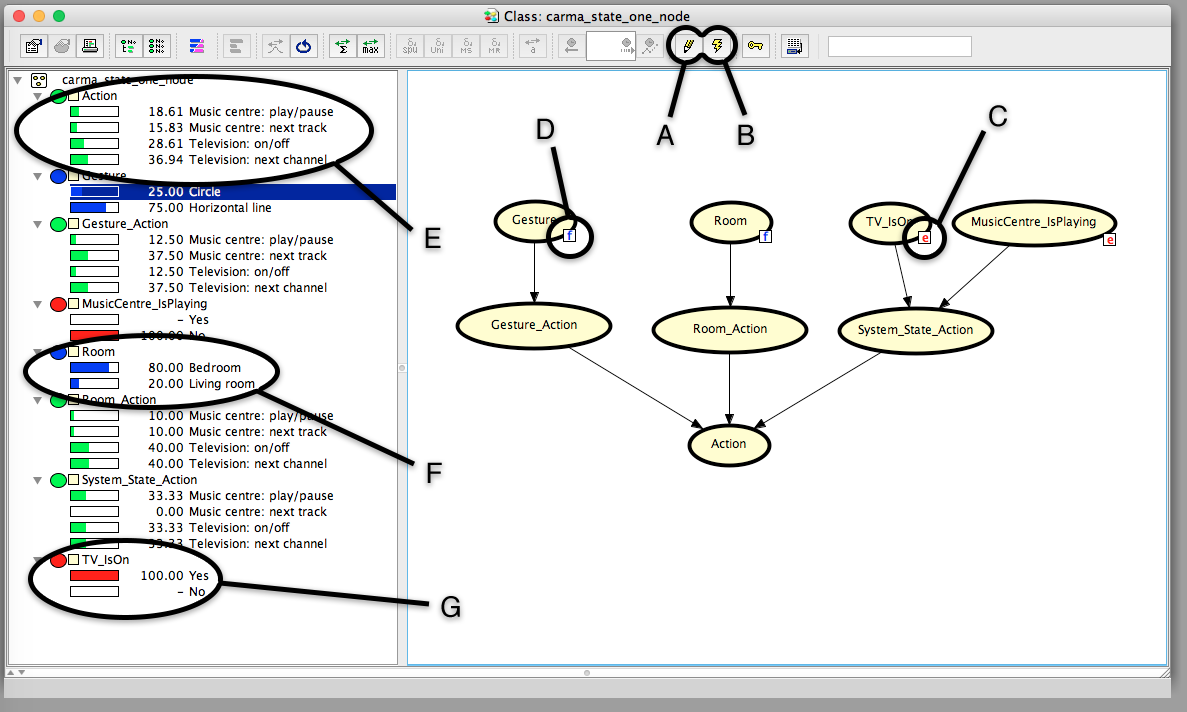
\includegraphics[width=\textwidth]{images/hugin-functionality-running}
\caption{Screenshot of Hugin while running the Bayesian network. The screenshot highlights important features of the software. Please see above for a description of the features.}
\label{fig:design:bayesian-network:hugin-functionality-running}
\end{figure}

\begin{figure}[h!]
\centering
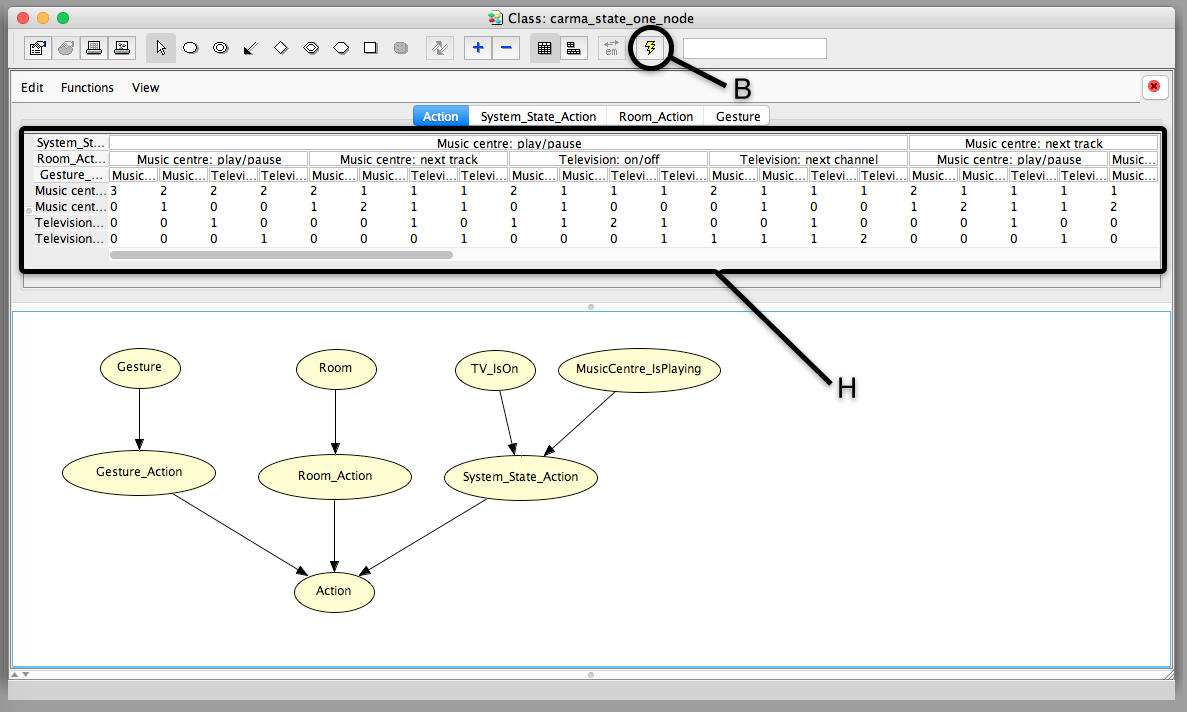
\includegraphics[width=\textwidth]{images/hugin-functionality-editing}
\caption{Screenshot of Hugin while editing the Bayesian network. The screenshot highlights important features of the software. Please see above for a description of the features.}
\label{fig:design:bayesian-network:hugin-functionality-editing}
\end{figure}

%%% Local Variables:
%%% mode: latex
%%% TeX-master: "../../master"
%%% End:
